\documentclass[11pt,a4paper]{article}
\usepackage[T1]{fontenc}
\usepackage[utf8]{inputenc}
\usepackage{lmodern}
\usepackage{textcomp}
\usepackage[left=1.8cm,right=1.8cm,top=2.3cm,bottom=2.2cm,headheight=14pt,headsep=8pt]{geometry}
\usepackage{multicol}
\usepackage{xcolor}
\usepackage{fancyhdr}
\usepackage{graphicx}
\usepackage{array}
\usepackage{amsmath,amssymb}
\usepackage{setspace}
\usepackage{longtable}
\graphicspath{{../}}
\definecolor{ygreen}{RGB}{46,139,87}
\renewcommand{\normalsize}{\fontsize{10.9}{13.4}\selectfont}
\renewcommand{\familydefault}{\rmdefault}
\setlength{\parindent}{0pt}
\setlength{\columnsep}{0.8cm}
\setlength{\columnseprule}{0.4pt}
\setlength{\multicolsep}{3pt plus 1pt minus 1pt}
\renewcommand{\textsubscript}[1]{\ensuremath{_{\text{\fontsize{8}{8}\selectfont #1}}}}
\renewcommand{\textsuperscript}[1]{\ensuremath{^{\text{\fontsize{8}{8}\selectfont #1}}}}
\newcommand{\diqqat}[1]{\par\smallskip\noindent\textbf{Diqqat!} #1\par\medskip}
\newcommand{\javob}{\par\smallskip\noindent\textbf{Javob:} \rule[-2pt]{7.5cm}{0.4pt}\par\smallskip\noindent\textbf{Diqqat!} Javobingizni javoblar varaqasiga ko`chirib yozing.\par\medskip}
\pagestyle{fancy}
\fancyhf{}
\renewcommand{\headrulewidth}{0.4pt}
\fancyhead[L]{\textit{Milliy sertifikat 2026. Kimyo}}
\fancyhead[R]{5-variant}
\fancyfoot[L]{\fontsize{8}{9}\selectfont \textcopyright{} Colba maktabi, 2026}
\fancyfoot[C]{\thepage}
\fancypagestyle{first}{\fancyhf{}\renewcommand{\headrulewidth}{0pt}\fancyfoot[L]{\fontsize{8}{9}\selectfont \textcopyright{} Colba maktabi, 2026}\fancyfoot[C]{\thepage}}
\begin{document}
\normalsize
\thispagestyle{first}
\noindent\fcolorbox{ygreen}{white}{\parbox{\dimexpr\linewidth-2\fboxsep-2\fboxrule\relax}{%
\textbf{\fontsize{13}{15}\selectfont Nazorat testi}\ \textit{\fontsize{10}{12}\selectfont $\cdot$ Aralash test $\cdot$ 5-variant}\hfill
\begin{tabular}[t]{@{}r@{}}\textit{Milliy sertifikat 2026. Kimyo}\\ \textbf{\textit{\fontsize{8}{9}\selectfont Vaqt:}} \textit{\fontsize{10}{12}\selectfont 180 daqiqa}\end{tabular}}}
\par\medskip
\noindent\textit{Davriy jadvaldan foydalanish mumkin.}
\par\medskip
\begin{multicols}{2}
\noindent\textbf{1.} Quyidagi tuzlarning qaysilari suvli eritmasi kislotali muhitga ega? 1) CH\textsubscript{3}COONa; 2) Na\textsubscript{2}SO\textsubscript{4}; 3) FeCl\textsubscript{3}; 4) Na\textsubscript{2}CO\textsubscript{3}

\noindent A)~\textsl{3} \hfill B)~\textsl{2} \hfill C)~\textsl{2, 4} \hfill D)~\textsl{1, 3}\par
\vspace{4pt}
\end{multicols}
\noindent\textbf{2.} N\textsubscript{2} + 3H\textsubscript{2} $\rightleftarrows$ 2NH\textsubscript{3} reaksiyasi 2 l hajmli idishda o`tkazildi. Moddalar miqdori jadvalda berilgan:
\begin{center}
\renewcommand{\arraystretch}{1.15}
\begin{tabular}{|c|c|c|c|}\hline
\textbf{Modda} & \textbf{N\textsubscript{2}} & \textbf{H\textsubscript{2}} & \textbf{NH\textsubscript{3}} \\ \hline
Boshlang`ich miqdor, mol & 2 & 6 & 0 \\ \hline
Muvozanatdagi miqdor, mol & --- & --- & 2 \\ \hline
\end{tabular}
\end{center}
Muvozanat \textbf{konstantasini (K) hisoblang.}

\noindent A)~\textsl{1,185} \hfill B)~\textsl{0,593} \hfill C)~\textsl{0,296} \hfill D)~\textsl{0,889}\par
\vspace{4pt}
\begin{multicols}{2}
\noindent\textbf{3.} 200 g 15\% li va 400 g 30\% li tuz eritmalari aralashtirildi. Hosil bo`lgan eritmaning massa \textbf{ulushini (\%) aniqlang.}

\noindent A)~\textsl{22,5} \hfill B)~\textsl{45} \hfill C)~\textsl{25} \hfill D)~\textsl{20}\par
\vspace{4pt}
\noindent\textbf{4.} VA guruh elementlarining vodorodli birikmalari qaynash haroratlari grafikda berilgan.
\begin{center}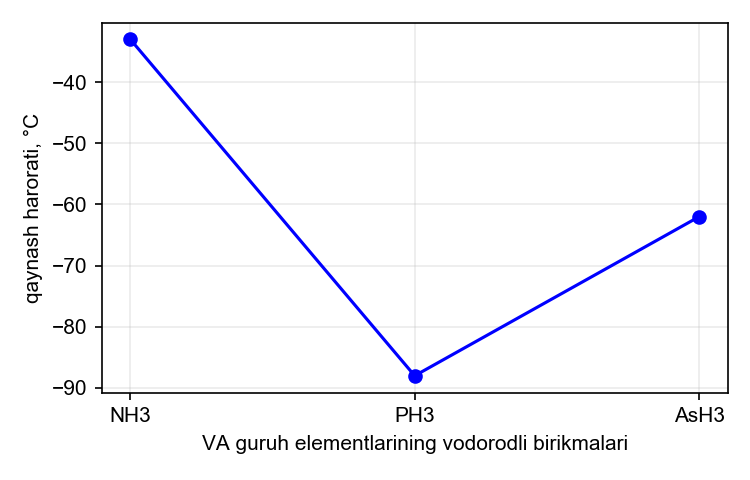
\includegraphics[width=0.86\linewidth]{rasmlar/gen/hy2_v05_0.png}\end{center}
NH\textsubscript{3} ning qaynash harorati yuqoriligining sababi nima?
\noindent A)~\textsl{Molekula massasi kattaligi}\par
\noindent B)~\textsl{Ion bog`lanish mavjudligi}\par
\noindent C)~\textsl{Molekulalararo vodorod bog`lanish borligi}\par
\noindent D)~\textsl{Kovalent bog` mustahkamligi}\par
\vspace{4pt}
\noindent\textbf{5.} 11,2 g Fe reaksiyaga kirishdi (Fe + 2HCl $\to$ FeCl\textsubscript{2} + H\textsubscript{2}). Ajralgan H\textsubscript{2} \textbf{hajmini (l, n.sh.) hisoblang} (unum 80\%).

\noindent A)~\textsl{3,58} \hfill B)~\textsl{4,48} \hfill C)~\textsl{7,17} \hfill D)~\textsl{1,79}\par
\vspace{4pt}
\noindent\textbf{6.} Jadvalda N elementining birikmalaridagi oksidlanish darajasi berilgan:
\begin{center}
\renewcommand{\arraystretch}{1.15}
\begin{tabular}{|c|c|}\hline
\textbf{Modda} & \textbf{Oksidlanish darajasi} \\ \hline
NO & +2 \\ \hline
NH\textsubscript{3} & -3 \\ \hline
HNO\textsubscript{3} & +5 \\ \hline
N\textsubscript{2} & 0 \\ \hline
\end{tabular}
\end{center}
Ushbu moddalardan nechtasida N elementi faqat oksidlovchi xossani namoyon qiladi? (N uchun eng past oksidlanish darajasi -3, eng yuqorisi +5)

\noindent A)~\textsl{2} \hfill B)~\textsl{3} \hfill C)~\textsl{0} \hfill D)~\textsl{1}\par
\vspace{4pt}
\noindent\textbf{7.} CuSO\textsubscript{4} ning suvli eritmasi inert elektrodlar bilan elektroliz qilinganda qaysi moddalar ajraladi?

\noindent\begin{tabular}{@{}p{0.47\linewidth}@{}p{0.47\linewidth}@{}}
A)~\textsl{Ag va O\textsubscript{2}} & B)~\textsl{H\textsubscript{2} va O\textsubscript{2}} \\
C)~\textsl{Cu va O\textsubscript{2}} & D)~\textsl{Zn, H\textsubscript{2} va O\textsubscript{2}} \\
\end{tabular}\par
\vspace{4pt}
\noindent\textbf{8.} 2SO\textsubscript{2} + O\textsubscript{2} $\rightleftarrows$ 2SO\textsubscript{3} + Q muvozanatni o`ngga siljitadigan \textbf{o`zgarishlarni toping}: 1) haroratni pasaytirish; 2) katalizator qo`shish; 3) bosimni pasaytirish; 4) bosimni oshirish.

\noindent A)~\textsl{1, 4} \hfill B)~\textsl{2, 3} \hfill C)~\textsl{1, 3, 4} \hfill D)~\textsl{1, 3}\par
\vspace{4pt}
\noindent\textbf{9.} Quyidagilarni jism va moddalarga ajrating: suv, stakan, oltingugurt, qaychi, grafit. Ulardan nechtasi modda?

\noindent A)~\textsl{4} \hfill B)~\textsl{2} \hfill C)~\textsl{5} \hfill D)~\textsl{3}\par
\vspace{4pt}
\noindent\textbf{10.} Xrom atomida d-pog`onachadagi elektronlar \textbf{sonini aniqlang} (\textit{Z} = 24).

\noindent A)~\textsl{6} \hfill B)~\textsl{4} \hfill C)~\textsl{7} \hfill D)~\textsl{5}\par
\vspace{4pt}
\noindent\textbf{11.} KMnO\textsubscript{4} + FeSO\textsubscript{4} + H\textsubscript{2}SO\textsubscript{4} $\to$ MnSO\textsubscript{4} + Fe\textsubscript{2}(SO\textsubscript{4})\textsubscript{3} + K\textsubscript{2}SO\textsubscript{4} + H\textsubscript{2}O reaksiya tenglamasini tenglang va barcha koeffitsiyentlar \textbf{yig`indisini aniqlang.}

\noindent A)~\textsl{37} \hfill B)~\textsl{36} \hfill C)~\textsl{35} \hfill D)~\textsl{38}\par
\vspace{4pt}
\noindent\textbf{12.} HC$\equiv$C--CH=CH\textsubscript{2} molekulasida sp\textsuperscript{2} gibridlangan uglerod atomlari nechta?

\noindent A)~\textsl{2} \hfill B)~\textsl{3} \hfill C)~\textsl{4} \hfill D)~\textsl{1}\par
\vspace{4pt}
\noindent\textbf{13.} H\textsubscript{2} + I\textsubscript{2} $\rightleftarrows$ 2HI reaksiyada muvozanat holatida [H\textsubscript{2}] = 0,5, [I\textsubscript{2}] = 1, [HI] = 1 mol/l. Muvozanat \textbf{konstantasini (K) hisoblang.}

\noindent A)~\textsl{4} \hfill B)~\textsl{1} \hfill C)~\textsl{2} \hfill D)~\textsl{0,667}\par
\vspace{4pt}
\noindent\textbf{14.} Nodir gazlar haqida qaysi fikrlar to`g`ri? 1) Nodir gazlar kimyoviy jihatdan juda faol; 2) Geliy eng yengil inert gaz; 3) Argon havoning hajmi bo`yicha eng ko`p uchraydigan inert gazi; 4) Geliyda 8 ta tashqi elektron bor

\noindent A)~\textsl{3} \hfill B)~\textsl{4} \hfill C)~\textsl{2, 3} \hfill D)~\textsl{2, 3, 4}\par
\vspace{4pt}
\noindent\textbf{15.} 10,1 g KNO\textsubscript{3} to`liq parchalanguncha qizdirildi. Qattiq qoldiq \textbf{massasini (g) aniqlang.}

\noindent A)~\textsl{8,5} \hfill B)~\textsl{10,1} \hfill C)~\textsl{17} \hfill D)~\textsl{4,25}\par
\vspace{4pt}
\noindent\textbf{16.} Qaysi juftliklar o`zaro reaksiyaga kirishadi? 1) Ag va H\textsubscript{2}SO\textsubscript{4}(suyult.); 2) CO\textsubscript{2} va CaO; 3) Na\textsubscript{2}CO\textsubscript{3} va HCl; 4) Fe va HCl

\noindent A)~\textsl{3, 4} \hfill B)~\textsl{1, 3, 4} \hfill C)~\textsl{1, 3} \hfill D)~\textsl{2, 3, 4}\par
\vspace{4pt}
\noindent\textbf{17.} 44,8 l (n.sh.) ammiakdan nitrat kislota olindi (jami unum 80\%). Kislota \textbf{massasini (g) aniqlang.}

\noindent A)~\textsl{126} \hfill B)~\textsl{100,8} \hfill C)~\textsl{201,6} \hfill D)~\textsl{50,4}\par
\vspace{4pt}
\noindent\textbf{18.} 0,3 mol NaOH tutgan eritmadan 0,15 mol CO\textsubscript{2} o`tkazildi. Hosil bo`lgan Na\textsubscript{2}CO\textsubscript{3} \textbf{massasini (g) aniqlang.}

\noindent A)~\textsl{31,8} \hfill B)~\textsl{7,95} \hfill C)~\textsl{12} \hfill D)~\textsl{15,9}\par
\vspace{4pt}
\noindent\textbf{19.} 11,7 g NaCl ga mo`l kons. H\textsubscript{2}SO\textsubscript{4} ta'sir ettirilib, ajralgan HCl 500 g suvda eritildi. Hosil bo`lgan xlorid kislota massa \textbf{ulushini (\%) aniqlang.}

\noindent A)~\textsl{1,44} \hfill B)~\textsl{1,46} \hfill C)~\textsl{2,88} \hfill D)~\textsl{0,72}\par
\vspace{4pt}
\noindent\textbf{20.} CH\textsubscript{4} + 2O\textsubscript{2} $\to$ CO\textsubscript{2} + 2H\textsubscript{2}O reaksiyasida 22,4 l (n.sh.) CH\textsubscript{4} ishtirok etdi. CO\textsubscript{2} \textbf{massasini (g) toping.}

\noindent A)~\textsl{88} \hfill B)~\textsl{44} \hfill C)~\textsl{22} \hfill D)~\textsl{66}\par
\vspace{4pt}
\noindent\textbf{21.} Alken, alkadiyen va alkinlar haqida qaysi fikrlar to`g`ri? 1) Propenga HBr birikishi Markovnikov qoidasiga bo`ysunadi; 2) Alkinlar uchun umumiy formula CnH\textsubscript{2}n+2; 3) Asetilenni Kucherov reaksiyasi bilan sirka aldegidiga aylantirish mumkin; 4) Asetilen Ag\textsubscript{2}O ning ammiakli eritmasi bilan cho`kma beradi (butin-2 beradi)

\noindent A)~\textsl{1, 3} \hfill B)~\textsl{1} \hfill C)~\textsl{1, 2} \hfill D)~\textsl{3}\par
\vspace{4pt}
\noindent\textbf{22.} Arenlar, neft va tabiiy gaz haqida qaysi fikrlar to`g`ri? 1) Neft fraksiyalaridan gazolin 150 \textdegree{}C gacha haydaladi; 2) Naftalin -- bir halqali aren; 3) Benzoldan nitrobenzol nitrolash bilan olinadi; 4) Toluol KMnO\textsubscript{4} bilan benzoy kislotagacha oksidlanadi

\noindent A)~\textsl{2, 3} \hfill B)~\textsl{1, 3, 4} \hfill C)~\textsl{1, 2, 3} \hfill D)~\textsl{3, 4}\par
\vspace{4pt}
\noindent\textbf{23.} Reaksiya tenglamasi: C\textsubscript{6}H\textsubscript{12}O\textsubscript{6} $\to$ 2C\textsubscript{2}H\textsubscript{5}OH + 2CO\textsubscript{2}. Reaksiyaga 360 g C\textsubscript{6}H\textsubscript{12}O\textsubscript{6} kirishdi (unum 75\%). C\textsubscript{2}H\textsubscript{5}OH \textbf{massasini (g) hisoblang.}

\noindent A)~\textsl{46} \hfill B)~\textsl{138} \hfill C)~\textsl{276} \hfill D)~\textsl{69}\par
\vspace{4pt}
\noindent\textbf{24.} To`yingan bir atomli aldegidning 5,8 g massasi Ag\textsubscript{2}O ning ammiakli eritmasi bilan oksidlanganda 21,6 g kumush ajraldi. Aldegidning molyar \textbf{massasini (g/mol) toping.}

\noindent A)~\textsl{116} \hfill B)~\textsl{29} \hfill C)~\textsl{72} \hfill D)~\textsl{58}\par
\vspace{4pt}
\noindent\textbf{25.} C\textsubscript{6}H\textsubscript{14} alkanning izomerlari soni nechta?

\noindent A)~\textsl{6} \hfill B)~\textsl{5} \hfill C)~\textsl{4} \hfill D)~\textsl{7}\par
\vspace{4pt}
\noindent\textbf{26.} Rasmdagi zanjirda C\textsubscript{2}H\textsubscript{4} dan C\textsubscript{2}H\textsubscript{6} olish uchun \textit{X} reagent va \textbf{sharoitni aniqlang.}
\begin{center}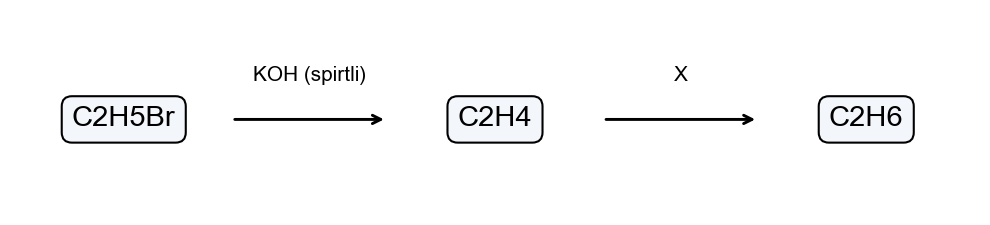
\includegraphics[width=0.86\linewidth]{rasmlar/gen/co_124463.png}\end{center}

\noindent\begin{tabular}{@{}p{0.47\linewidth}@{}p{0.47\linewidth}@{}}
A)~\textsl{H\textsubscript{2}, kat.} & B)~\textsl{HNO\textsubscript{3}, H\textsubscript{2}SO\textsubscript{4}} \\
C)~\textsl{H\textsubscript{2}, Ni} & D)~\textsl{C\textsubscript{2}H\textsubscript{5}OH, H\textsubscript{2}SO\textsubscript{4}} \\
\end{tabular}\par
\vspace{4pt}
\noindent\textbf{27.} 34,2 g maltoza to`liq gidrolizlanib, hosil bo`lgan mahsulot Ag\textsubscript{2}O ning ammiakli eritmasi bilan oksidlandi. Ajralgan kumush \textbf{massasini (g) aniqlang.}

\noindent A)~\textsl{43,2} \hfill B)~\textsl{21,6} \hfill C)~\textsl{86,4} \hfill D)~\textsl{10,8}\par
\vspace{4pt}
\noindent\textbf{28.} Reaksiya tenglamasi: NH\textsubscript{2}CH\textsubscript{2}COOH + NaOH $\to$ NH\textsubscript{2}CH\textsubscript{2}COONa + H\textsubscript{2}O. Reaksiyaga 15 g NH\textsubscript{2}CH\textsubscript{2}COOH kirishdi. NaOH \textbf{massasini (g) hisoblang.}

\noindent A)~\textsl{16} \hfill B)~\textsl{4} \hfill C)~\textsl{12} \hfill D)~\textsl{8}\par
\vspace{4pt}
\noindent\textbf{29.} C\textsubscript{2}H\textsubscript{2} + H\textsubscript{2}O (Hg\textsuperscript{2+}) reaksiyasi natijasida qaysi organik modda hosil bo`ladi?

\noindent\begin{tabular}{@{}p{0.47\linewidth}@{}p{0.47\linewidth}@{}}
A)~\textsl{benzol} & B)~\textsl{benzoy kislota} \\
C)~\textsl{sirka aldegid} & D)~\textsl{asetilen} \\
\end{tabular}\par
\vspace{4pt}
\noindent\textbf{30.} Qum va suv aralashmasi ni ajratish uchun qaysi usul mos?
\noindent A)~\textsl{ajratgich voronka}\par
\noindent B)~\textsl{suvda eritib, filtrlash, so`ng bug`latish}\par
\noindent C)~\textsl{distillash (fraksiyalab haydash)}\par
\noindent D)~\textsl{filtrlash}\par
\vspace{4pt}
\noindent\textbf{31.} Rasmdagi tajribada efirlanish reaksiyasida konsentrlangan H\textsubscript{2}SO\textsubscript{4} qanday vazifani bajaradi?
\begin{center}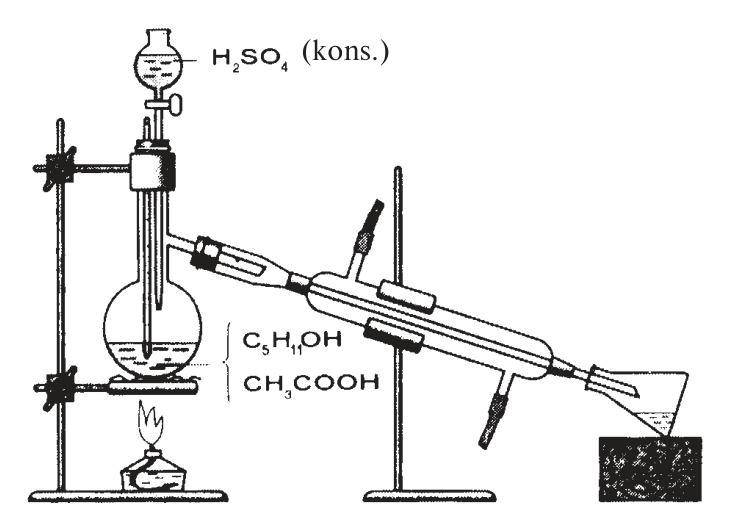
\includegraphics[width=0.86\linewidth]{rasmlar/darslik/d_efir.png}\end{center}
\noindent A)~\textsl{oksidlovchi}\par
\noindent B)~\textsl{katalizator va suv tortuvchi}\par
\noindent C)~\textsl{reaksiya mahsuloti}\par
\noindent D)~\textsl{faqat erituvchi}\par
\vspace{4pt}
\end{multicols}
\noindent\textbf{32.} Uch probirkada (\textit{X}, \textit{Y}, \textit{Z}) AlCl\textsubscript{3}, MgCl\textsubscript{2}, KCl eritmalari bor (tartibsiz). Ularga NaOH ta'sir ettirildi. Kuzatuvlar jadvalda:
\begin{center}
\renewcommand{\arraystretch}{1.15}
\begin{tabular}{|c|c|c|}\hline
\textbf{Probirka} & \textbf{oz miqdor NaOH} & \textbf{mo`l miqdor NaOH} \\ \hline
\textit{X} & o`zgarish yo`q & --- \\ \hline
\textit{Y} & oq cho`kma & cho`kma mo`l ishqorda eriydi \\ \hline
\textit{Z} & oq cho`kma & cho`kma erimaydi \\ \hline
\end{tabular}
\end{center}
\textit{X}, \textit{Y}, \textit{Z} probirkalardagi \textbf{moddalarni aniqlang.}
\noindent A)~\textsl{\textit{X} -- MgCl\textsubscript{2}, \textit{Y} -- AlCl\textsubscript{3}, \textit{Z} -- KCl}\par
\noindent B)~\textsl{\textit{X} -- AlCl\textsubscript{3}, \textit{Y} -- KCl, \textit{Z} -- MgCl\textsubscript{2}}\par
\noindent C)~\textsl{\textit{X} -- KCl, \textit{Y} -- AlCl\textsubscript{3}, \textit{Z} -- MgCl\textsubscript{2}}\par
\noindent D)~\textsl{\textit{X} -- KCl, \textit{Y} -- MgCl\textsubscript{2}, \textit{Z} -- AlCl\textsubscript{3}   ---}\par
\vspace{4pt}
\begin{multicols}{2}
\end{multicols}
\medskip
\noindent\setlength{\fboxsep}{0pt}\fbox{\begin{tabular}{p{0.74\linewidth}|p{0.2\linewidth}}
\parbox[t]{0.72\linewidth}{\vspace{3pt}\textbf{Topshiriqlar (33--35) va javob variant (A--F)larini o`zaro to`g`ri moslashtiring.} Etanol va fenoldan iborat 14 g aralashma natriy bilan to`liq reaksiyaga kirishganda 2,24 l (n.sh.) vodorod ajraldi. Xuddi shu massadagi aralashma NaOH eritmasi bilan (faqat fenol) va bromli suv bilan (faqat fenol) ham reaksiyaga kirishadi.
\vspace{3pt}} & \parbox[t]{0.19\linewidth}{\vspace{3pt}A~\textsl{4}\\[3pt]
B~\textsl{8}\\[3pt]
C~\textsl{2}\\[3pt]
D~\textsl{67,14}\\[3pt]
E~\textsl{59,58}\\[3pt]
F~\textsl{29,79}}\\ \hline
\parbox[t]{0.72\linewidth}{\vspace{2pt}\textbf{33. Aralashmadagi fenol massa ulushini (\%) aniqlang.}\vspace{2pt}} & \\ \hline
\parbox[t]{0.72\linewidth}{\vspace{2pt}\textbf{34. Fenolni to`liq neytrallash uchun zarur NaOH massasini (g) aniqlang.}\vspace{2pt}} & \\ \hline
\parbox[t]{0.72\linewidth}{\vspace{2pt}\textbf{35. Mo`l bromli suv bilan reaksiyada hosil bo`lgan tribromfenol massasini (g) aniqlang (reaksiya unumi 90\%).}\vspace{2pt}} & 
\end{tabular}}
\par\bigskip
\noindent\textbf{36.} Fe + H\textsubscript{2}SO\textsubscript{4} $\to$ Fe\textsubscript{2}(SO\textsubscript{4})\textsubscript{3} + SO\textsubscript{2} + H\textsubscript{2}O reaksiya tenglamasini elektron balans usulida tenglang va barcha koeffitsiyentlar \textbf{yig`indisini aniqlang.}
\javob
\noindent\textbf{37.} Reaksiya 30 \textdegree{}C da 72 minutda tugaydi. $\gamma$ = 3. Harorat 20 \textdegree{}C ga oshirilib, reagentlardan birining konsentratsiyasi 2 marta oshirildi (reaksiya shu modda bo`yicha 1-tartibli). Reaksiya necha minutda tugaydi?
\javob
\noindent\textbf{38.} 6,2 g fosfor yondirib hosil bo`lgan oksid suvda eritildi, so`ng eritmaga 0,5 mol NaOH qo`shildi (NaOH : H\textsubscript{3}PO\textsubscript{4} = 2,5 : 1). Hosil bo`lgan tuzlar umumiy \textbf{massasini (g) toping.}
\javob
\noindent\textbf{39.} 180 g glyukoza spirtli bijg`ish natijasida etanolga (unum 90\%), hosil bo`lgan etanol esa sirka kislotagacha (unum 80\%) aylantirildi. Olingan kislotani to`liq neytrallash uchun NaOH ning \textbf{massasini (g) toping.}
\javob
\noindent\textbf{40.} 24,6 g nitrobenzol anilinga qaytarildi (unum 90\%), hosil bo`lgan anilin mo`l bromli suv bilan reaksiyaga kirishdi (unum 80\%). Hosil bo`lgan 2,4,6-tribromanilin (M = 330 g/mol) \textbf{massasini (g) toping.}
\javob
\par\bigskip\begin{center}\textbf{\fontsize{13}{15}\selectfont YOZMA ISH}\end{center}
\noindent\textbf{41.} \textbf{Topshiriqni bajarish jarayonida barcha reaksiya tenglamalarini yozing. Miqdoriy va arifmetik hisoblashlarni (unga asos bo`lgan usul yoki formulani ko`rsatgan holda) uzviy ketma-ketlikda bajaring.}\par\smallskip
2 l hajmli idishda N\textsubscript{2} + 3H\textsubscript{2} $\rightleftarrows$ 2NH\textsubscript{3} reaksiyasi muvozanat holatiga keldi. Muvozanatda idishda 4 mol N\textsubscript{2}, 4 mol H\textsubscript{2} va 8 mol NH\textsubscript{3} bor.\par
\noindent 1)Muvozanat konstantasini (K) hisoblang.\par
\noindent 2)Azot va vodorodning boshlang`ich konsentratsiyalarini (mol/l) aniqlang. H\textsubscript{2} ning boshlang`ich massasini (g) ham toping.\par
\noindent 3)Vodorodning necha foizi reaksiyaga kirishgan?\par
\noindent 4)Hosil bo`lgan ammiakning hammasi 200 g suvda eritildi. Eritmadagi ammiakning massa ulushini (\%) hisoblang. Ajralgan NH\textsubscript{3} hajmini (l, n.sh.) ham toping.\par
\noindent 5)Shu eritmani (NH\textsubscript{4})\textsubscript{2}SO\textsubscript{4} hosil bo`lguncha neytrallash uchun 20\% li H\textsubscript{2}SO\textsubscript{4} eritmasidan necha gramm kerak? Idish hajmi 2 marta kamaytirilsa, to`g`ri reaksiya tezligi (elementar deb hisoblang) necha marta ortadi?\par
\diqqat{Mazkur topshiriq kengaytirilgan javobni talab etib, uning yechilish usuli va shu usul asosidagi barcha hisoblash amallari javoblar varaqasida aks etishi lozim.}
\noindent\textbf{42.} Quyidagi o`zgarishlar zanjirida \textit{X}, \textit{Y}, \textit{Z} noma'lum organik moddalar:\par
\[\setlength{\fboxsep}{0pt}\text{C\textsubscript{12}H\textsubscript{22}O\textsubscript{11}}\xrightarrow{\text{H\textsubscript{2}O, H\textsuperscript{+}}}\text{\textit{X}}\xrightarrow{\text{bijg`ish}}\text{\textit{Y}}\xrightarrow{\text{CuO, t\textdegree{}}}\text{\textit{Z}}\xrightarrow{\text{Ag\textsubscript{2}O, NH\textsubscript{3}}}\text{CH\textsubscript{3}COOH}\]
\noindent 1)C\textsubscript{12}H\textsubscript{22}O\textsubscript{11} $\to$ \textit{X} : reaksiya tenglamasini yozing; hosil bo`lgan moddani nomlang.\par
\noindent 2)\textit{X} $\to$ \textit{Y} : reaksiya tenglamasini yozing; hosil bo`lgan moddani nomlang.\par
\noindent 3)\textit{Y} $\to$ \textit{Z} : reaksiya tenglamasini yozing; hosil bo`lgan moddani nomlang.\par
\noindent 4)\textit{Z} $\to$ CH\textsubscript{3}COOH : reaksiya tenglamasini yozing; hosil bo`lgan moddani nomlang.\par
\diqqat{Mazkur topshiriq kengaytirilgan javobni talab etib, uning yechilish usuli va shu usul asosidagi barcha hisoblash amallari javoblar varaqasida aks etishi lozim.}
\noindent\textbf{43.} \textbf{Topshiriqni bajarish jarayonida barcha reaksiya tenglamalarini yozing. Miqdoriy va arifmetik hisoblashlarni (unga asos bo`lgan usul yoki formulani ko`rsatgan holda) uzviy ketma-ketlikda bajaring.}\par\smallskip
Laboratoriyada 1--4-raqamli probirkalarda tartibsiz holda glyukoza, kraxmal kleysteri, tuxum oqsili va glitserin eritmalari bor. Ularni aniqlash uchun quyidagi tajribalar o`tkazildi:\par
a) 1-probirkaga yodning spirtdagi eritmasidan qo`shildi --- eritma ko`k rangga bo`yaldi.\par
b) 2-probirkaga ishqor eritmasi va bir necha tomchi mis(II)-sulfat qo`shilganda eritma qizil-binafsha rangga bo`yaldi; boshqa porsiyasiga konsentrlangan HNO\textsubscript{3} qo`shib qizdirilganda sariq rang paydo bo`ldi.\par
c) 3- va 4-probirkalarga yangi cho`ktirilgan Cu(OH)\textsubscript{2} qo`shilganda ikkalasida ham cho`kma erib, ko`k eritma hosil bo`ldi. 3-probirka qizdirilganda avval sariq, so`ng qizil cho`kma tushdi, 4-probirkada esa o`zgarish bo`lmadi.\par
\noindent 1)Glyukozaning Cu(OH)\textsubscript{2} bilan reaksiya tenglamasini yozing. 9 g glyukoza mo`l Cu(OH)\textsubscript{2} bilan qizdirilganda hosil bo`lgan qizil cho`kmaning massasini (g) hisoblang.\par
\noindent 2)1--4-probirkalardagi moddalarni aniqlang (probirka raqami bilan moslab yozing).\par
\noindent 3)a), b) va c) bo`yicha kuzatilgan rang o`zgarishlarining sababini tushuntiring: qaysi funksional guruh yoki bog` bilan bog`liq?\par
\noindent 4)Tajribada probirkani qizdirish va konsentrlangan HNO\textsubscript{3} bilan ishlashda qanday xavfsizlik qoidalariga rioya qilish kerak? Kamida uchta qoida yozing.\par
\noindent 5)Glyukozaning (9 g) spirtli bijg`ishida ajraladigan CO\textsubscript{2} hajmini (l, n.sh.) hisoblang.\par
\diqqat{Mazkur topshiriq kengaytirilgan javobni talab etib, uning yechilish usuli va shu usul asosidagi barcha hisoblash amallari javoblar varaqasida aks etishi lozim.}
\newpage
\noindent\textbf{\fontsize{13}{15}\selectfont Nazorat testi}\ \textit{$\cdot$ 5-variant}\hfill \textbf{Javoblar kaliti}\par\smallskip\hrule\smallskip
\textit{Faqat o`qituvchi uchun.}\par\medskip
\noindent\textbf{1--32-savollar}\par\smallskip
\noindent\begin{tabular}{|c|c|c|c|c|c|c|c|c|c|c|c|c|c|c|c|}\hline
\textbf{1} & \textbf{2} & \textbf{3} & \textbf{4} & \textbf{5} & \textbf{6} & \textbf{7} & \textbf{8} & \textbf{9} & \textbf{10} & \textbf{11} & \textbf{12} & \textbf{13} & \textbf{14} & \textbf{15} & \textbf{16}\\\hline
\textsl{A} & \textsl{B} & \textsl{C} & \textsl{C} & \textsl{A} & \textsl{D} & \textsl{C} & \textsl{A} & \textsl{D} & \textsl{D} & \textsl{B} & \textsl{A} & \textsl{C} & \textsl{C} & \textsl{A} & \textsl{D}\\\hline
\textbf{17} & \textbf{18} & \textbf{19} & \textbf{20} & \textbf{21} & \textbf{22} & \textbf{23} & \textbf{24} & \textbf{25} & \textbf{26} & \textbf{27} & \textbf{28} & \textbf{29} & \textbf{30} & \textbf{31} & \textbf{32}\\\hline
\textsl{B} & \textsl{D} & \textsl{A} & \textsl{B} & \textsl{A} & \textsl{B} & \textsl{B} & \textsl{D} & \textsl{B} & \textsl{C} & \textsl{A} & \textsl{D} & \textsl{C} & \textsl{D} & \textsl{B} & \textsl{C}\\\hline
\end{tabular}\par\medskip
\noindent\textbf{33--35-savollar}\par\smallskip
\noindent\begin{tabular}{|c|c|c|}\hline \textbf{No} & \textbf{Javob} & \textbf{Qiymat}\\\hline
33 & \textsl{D} & 67,14\\\hline
34 & \textsl{A} & 4\\\hline
35 & \textsl{F} & 29,79\\\hline
\end{tabular}\par\medskip
\noindent\textbf{36--40-savollar}\par\smallskip
\noindent\begin{tabular}{|c|c|}\hline \textbf{No} & \textbf{To`g`ri javob}\\\hline
36 & 18\\\hline
37 & 4\\\hline
38 & 30,6\\\hline
39 & 57,6\\\hline
40 & 47,52\\\hline
\end{tabular}\par\medskip
\noindent\textbf{41--43-topshiriqlar: qisqa yechim}\par\smallskip
\noindent\textbf{41-topshiriq.}\par
\noindent 1) Muvozanat konsentratsiyalari: [N\textsubscript{2}] = 2, [H\textsubscript{2}] = 2, [NH\textsubscript{3}] = 4 mol/l; K = [NH\textsubscript{3}]\textsuperscript{2}/([N\textsubscript{2}]$\cdot$[H\textsubscript{2}]\textsuperscript{3}) = \textbf{1}\par
\noindent 2) NH\textsubscript{3} 8 mol hosil bo`lgan $\to$ N\textsubscript{2} sarfi 4 mol, H\textsubscript{2} sarfi 12 mol; boshlang`ich N\textsubscript{2} = \textbf{4 mol/l}, H\textsubscript{2} = \textbf{8 mol/l}; m(H\textsubscript{2}) = 16$\cdot$2 = \textbf{32 g}\par
\noindent 3) $\alpha$(H\textsubscript{2}) = 12/16 = \textbf{75\%}\par
\noindent 4) m(NH\textsubscript{3}) = 8$\cdot$17 = 136 g; $\omega$ = 136/(136 + 200) = \textbf{40,48\%}; \textit{V} = 8$\cdot$22,4 = \textbf{179,2 l}\par
\noindent 5) 2NH\textsubscript{3} + H\textsubscript{2}SO\textsubscript{4} $\to$ (NH\textsubscript{4})\textsubscript{2}SO\textsubscript{4}: H\textsubscript{2}SO\textsubscript{4} 4 mol = 392 g; eritma 392/0,2 = \textbf{1960 g}; v \textasciitilde{} [N\textsubscript{2}][H\textsubscript{2}]\textsuperscript{3}: 2\textsuperscript{4} = \textbf{16 marta}\par
\noindent Jami: M 15 + A 10 = 25 ball.\par
\noindent\textbf{42-topshiriq.}\par
\noindent 1) C\textsubscript{12}H\textsubscript{22}O\textsubscript{11} + H\textsubscript{2}O, H\textsuperscript{+} $\to$ C\textsubscript{6}H\textsubscript{12}O\textsubscript{6} (glyukoza)\par
\noindent 2) C\textsubscript{6}H\textsubscript{12}O\textsubscript{6} + bijg`ish $\to$ C\textsubscript{2}H\textsubscript{5}OH (etanol)\par
\noindent 3) C\textsubscript{2}H\textsubscript{5}OH + CuO, t\textdegree{} $\to$ CH\textsubscript{3}CHO (sirka aldegid (etanal))\par
\noindent 4) CH\textsubscript{3}CHO + Ag\textsubscript{2}O, NH\textsubscript{3} $\to$ CH\textsubscript{3}COOH (sirka kislota)\par
\noindent Jami 25 ball.\par
\noindent\textbf{43-topshiriq.}\par
\noindent 1) CH\textsubscript{2}OH--(CHOH)\textsubscript{4}--CHO + 2Cu(OH)\textsubscript{2} $\to$ CH\textsubscript{2}OH--(CHOH)\textsubscript{4}--COOH + Cu\textsubscript{2}O$\downarrow$ + 2H\textsubscript{2}O; n(glyukoza) = 9/180 = 0,05 mol $\to$ Cu\textsubscript{2}O 0,05 mol $\cdot$ 144 = \textbf{7,2 g}\par
\noindent 2) 1 --- kraxmal kleysteri (yod bilan ko`k); 2 --- tuxum oqsili (biuret va ksantoprotein reaksiyalari); 3 --- glyukoza; 4 --- glitserin\par
\noindent 3) a) kraxmal yod bilan ko`k rang beradi. b) oqsil: ishqoriy muhitda CuSO\textsubscript{4} bilan qizil-binafsha rang --- peptid bog` (--CO--NH--) uchun biuret reaksiyasi; kons. HNO\textsubscript{3} bilan sariq rang --- aromatik halqali aminokislota qoldiqlari (ksantoprotein). c) glyukoza va glitserin Cu(OH)\textsubscript{2} ni eritib ko`k kompleks hosil qiladi (ko`p atomli spirt guruhlari); faqat glyukozada aldegid guruh bor, qizdirilganda Cu\textsubscript{2}O gacha qaytariladi\par
\noindent 4) Probirka qisqichda tik, og`zi odamga qaratilmagan holda ohista qizdiriladi; kons. kislotani ko`zoynak va qo`lqopda ehtiyotlik bilan ishlatish, teriga tushsa ko`p suv bilan yuvish; reaktivlarni tatib ko`rmaslik; ortiqcha reaktivni idishga qaytarmaslik; kichik miqdorda ishlash\par
\noindent 5) C\textsubscript{6}H\textsubscript{12}O\textsubscript{6} $\to$ 2C\textsubscript{2}H\textsubscript{5}OH + 2CO\textsubscript{2}: n(CO\textsubscript{2}) = 2$\cdot$0,05 = 0,1 mol $\to$ \textbf{2,24 l}\par
\noindent Jami: M 15 + A 10 = 25 ball.\par
\par\bigskip\noindent\textbf{Mavzular taqsimoti}\par\smallskip
{\small\noindent\begin{longtable}{|c|p{7.2cm}|p{5.4cm}|c|}\hline \textbf{No} & \textbf{Mavzu} & \textbf{Tekshiriladigan ko`nikma} & \textbf{Ball}\\\hline
1 & 9-sinf (gidroliz); Tirkashev IV bob & Bilim va tushunish & 1\\\hline
2 & Tirkashev VI bob (muvozanat, jadval) & Jadval tahlili & 1\\\hline
3 & Tirkashev III bob (eritmalar) & Hisoblash va masala yechish & 1\\\hline
4 & 8-sinf (vodorod bog`lanish, grafik) & Grafik tahlili & 1\\\hline
5 & 8-sinf; 9-sinf (stexiometriya) & Hisoblash va masala yechish & 1\\\hline
6 & Tirkashev \textit{V} bob (OQR, jadval) & Jadval tahlili & 1\\\hline
7 & 11-sinf 8-bob; Tirkashev \textit{V} bob (elektroliz) & Bilim va tushunish & 1\\\hline
8 & Tirkashev VI bob (Le-Shatelye) & Bilim va tushunish & 1\\\hline
9 & 7-sinf (jism va modda) & Bilim va tushunish & 1\\\hline
10 & Tirkashev I bob; 8-sinf (elektron konfiguratsiya) & Bilim va tushunish & 1\\\hline
11 & Tirkashev \textit{V} bob; 11-sinf 7-bob (OQR tenglash) & Hisoblash va masala yechish & 1\\\hline
12 & 10-sinf \S{}17 & Bilim va tushunish & 1\\\hline
13 & Tirkashev VI bob (kimyoviy muvozanat) & Hisoblash va masala yechish & 1\\\hline
14 & Tashev (nodir gazlar); 8-sinf & Bilim va tushunish & 1\\\hline
15 & Tashev (nitratlar termik parchalanishi) & Hisoblash va masala yechish & 1\\\hline
16 & 9-sinf; Tashev (anorganik birikmalar xossalari) & Bilim va tushunish & 1\\\hline
17 & Tashev (HNO\textsubscript{3} olinishi) & Hisoblash va masala yechish & 1\\\hline
18 & 9-sinf (uglerod (IV) oksid) & Hisoblash va masala yechish & 1\\\hline
19 & Tashev (HCl olinishi) & Hisoblash va masala yechish & 1\\\hline
20 & 10-sinf (alkan, hisob) & Hisoblash va masala yechish & 1\\\hline
21 & 10-sinf (mavzuga oid paragraflar); Abdusamatov & Bilim va tushunish & 1\\\hline
22 & 10-sinf (mavzuga oid paragraflar); Abdusamatov & Bilim va tushunish & 1\\\hline
23 & 10-sinf (spirt, hisob) & Hisoblash va masala yechish & 1\\\hline
24 & 10-sinf \S{}24 & Hisoblash va masala yechish & 1\\\hline
25 & 10-sinf \S{}6, \S{}12, \S{}20, \S{}28 (izomeriya) & Bilim va tushunish & 1\\\hline
26 & 10-sinf (organik moddalarning o`zaro bog`lanishi) & Rasm bo`yicha tahlil & 1\\\hline
27 & 10-sinf \S{}31 (maltoza) & Hisoblash va masala yechish & 1\\\hline
28 & 10-sinf (amin, hisob) & Hisoblash va masala yechish & 1\\\hline
29 & 10-sinf (olinish usullari) & Bilim va tushunish & 1\\\hline
30 & 7-sinf (aralashmalarni ajratish usullari) & Bilim va tushunish & 1\\\hline
31 & 10-sinf (efirlanish, 8-rasm) & Rasm bo`yicha tahlil & 1\\\hline
32 & 7--10-sinf va Tashev (laboratoriya ishlari, sifat reaksiyalar) & Jadval tahlili & 1\\\hline
33--35 & Aralash masala (moslashtirish) & Ko`p bosqichli hisob & 3\\\hline
36--40 & Qisqa javobli masalalar & Hisoblash & 5\\\hline
41--43 & Yozma ish & Usul va hisob (M, A) & 75\\\hline
\end{longtable}}
\end{document}
